\begin{enumerate}
\item
In triangle $ABC$, $AB = 1$, $BC = 1$, and $\angle A = \dfrac{\pi}{3}$ radians. Find $CA$ and $\angle B$.
\newline
\begin{center}
	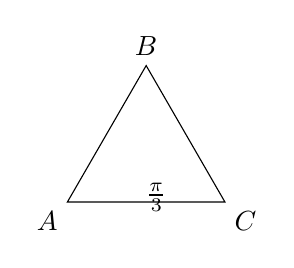
\begin{tikzpicture}
		\coordinate (A) at (-1,0);
		\coordinate (B) at (0, 1.732);
		\coordinate (C) at (1,0);

		\draw (A) node[below left]{$A$}
		-- (B) node[above]{$B$}
		-- (C) node[below right]{$C$}
		-- cycle;
		\tkzMarkAngle[size=0.8](C,A,B)
		\tkzLabelAngle [pos = 0.5](C,A,B){$\frac{\pi}{3}$}
		
		\tkzMarkAngle[size=0.8](B,C,A)
		
		\tkzMarkSegment[color=blue,pos=.5,mark=|](A,B)
		\tkzMarkSegment[color=blue,pos=.5,mark=|](B,C)  
	\end{tikzpicture}
\end{center}
Since we know the triangle is isosceles since $BC = AB$, we see that $\angle C = \frac{\pi}{3}$ radians. But that means that $\angle B = \frac{\pi}{3}$ radians as well (since the three internal angles must sum to $\pi$) and so the triangle is equilateral. Consequently every side has a length of 1, and so $AC = 1$. In fact the picture should look like the following.
\begin{center}
	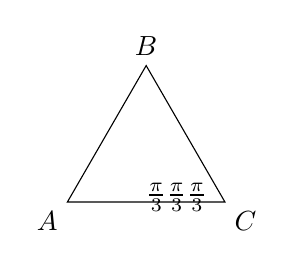
\begin{tikzpicture}
		\coordinate (A) at (-1,0);
		\coordinate (B) at (0, 1.732);
		\coordinate (C) at (1,0);

		\draw (A) node[below left]{$A$}
		-- (B) node[above]{$B$}
		-- (C) node[below right]{$C$}
		-- cycle;
		\tkzMarkAngle[size=0.6](C,A,B)
		\tkzLabelAngle [pos = 0.4](C,A,B){$\frac{\pi}{3}$}
		
		\tkzMarkAngle[size=0.6](B,C,A)
		\tkzLabelAngle [pos = 0.4](B,C,A){$\frac{\pi}{3}$}
		
		\tkzMarkAngle[size=0.6](A,B,C)
		\tkzLabelAngle [pos = 0.4](A,B,C){$\frac{\pi}{3}$}

		\tkzMarkSegment[color=blue,pos=.5,mark=|](A,B)
		\tkzMarkSegment[color=blue,pos=.5,mark=|](B,C)  
		\tkzMarkSegment[color=blue,pos=.5,mark=|](C,A)  
	\end{tikzpicture}
\end{center}
\item
In triangle $ABC$, $AB = 2$, $BC = 2$ and $AC = 3$. Find the angles of the triangle.
\newline
\begin{center}
	\begin{tikzpicture}
		\coordinate (A) at (-1.5,0);
		\coordinate (B) at (0, 1.732);
		\coordinate (C) at (1.5,0);

		\draw (A) node[below left]{$A$}
		-- (B) node[above]{$B$}
		-- (C) node[below right]{$C$}
		-- cycle;
		
		\tkzMarkSegment[color=blue,pos=.5,mark=|](A,B)
		\tkzMarkSegment[color=blue,pos=.5,mark=|](B,C) 

		\tkzLabelSegment[midway, sloped, above left](A,B){2}
		\tkzLabelSegment[midway, sloped, above right](B,C){2}
		\tkzLabelSegment[midway, below](A,C){3}
	\end{tikzpicture}
\end{center}
By the law of cosines we have
\[
9 = 8 -8\cos(\angle B),
\]
or equivalently
\[
\cos(\angle B) = -\frac{1}{8}.
\]
\[
\angle B \approx 1.696 \text{ radians}.
\]
Then since $\angle A = \angle C$ and the three angles sum to $\pi$, we have
\[
\angle A = \angle C \approx 0.723 \text{ radians}.
\]
\end{enumerate}